%Review of existing harmonic excitation.
%	Nonlinear Systems
%		Traditional Metrics (THD, IMD)
%		Minimisation of Nonlinear Distortion
%		Advent of "Nonlinear Niceness"
%	Timbre of nonlinear distortions (Martens and Marui type shit)
%	Uses of Harmonic Excitation
%	Harmonic Generation Methods
%		Static Nonlinearities
%		Bandwidth Extension (high frequency reconstruction)
%		Individual Harmonic Generation (SMC paper)
%		Psychoacoustic Enhancers

\chapter{Harmonic Excitation}
\label{chap:Excitation}

\section{Introduction}
\label{sec:Excitation-Introduction}
	\note{Harmonic excitation is of the chain. Look I wrote a paper about it \citep{enderby2013methods}.}

\section{Nonlinear Systems}
\label{sec:Excitation-NonlinearSystems}
	\note
	{
		THD and IMD are rubbish but served some purpose in the olden days. Some more metrics were made but they were still only concerned with minimising distortion \citep{lee2003auditory, geddes2003auditory, tan2004predicting}. \citet{voishvillo2006assessment} summarises a lot of metrics nicely. Then some bloke decided distortion was cool.
	}

\section{Timbre of Nonlinear Distortion}
\label{sec:Excitation-Timbre}
	\note
	{
		Marui and Martens did some of this \citep{marui2005timbre, marui2005constructing, marui2005predicting}.
	}

\section{Uses of Harmonic Excitation}
\label{sec:Excitation-Uses}
	\note
	{
		Psychoacoustic reproduction of low frequency signals on small loudspeakers as done by \citet{larsen2002reproducing} and \citet{gan2001virtual}.

		Reconstruction of high frequency components after lossy data compression \citep{friedrich2007spectral, nagel2009a, nagel2010a, valin2000bandwidth, dietz2002spectral, larsen2002efficient, sha2010high}.
	}

\section{Harmonic Generation Methods}
\label{sec:Excitation-Methods}
	\note{I like to generate harmonics, basically a nonlinear process}

	\subsection{Static Nonlinearities}
	\label{sec:Excitation-Statics}
		\note{DAFx Paper}

	\subsection{Bandwidth Extension}
	\label{sec:Excitation-BWE}
		\note
		{
			A nice summary in \citet{larsen2004audio}.

			Look at Figure \ref{fig:SpectralFolding} 'aint it fancy.
		}

		\begin{figure}[h!]
			\centering
			\subfloat[Spectral Folding]{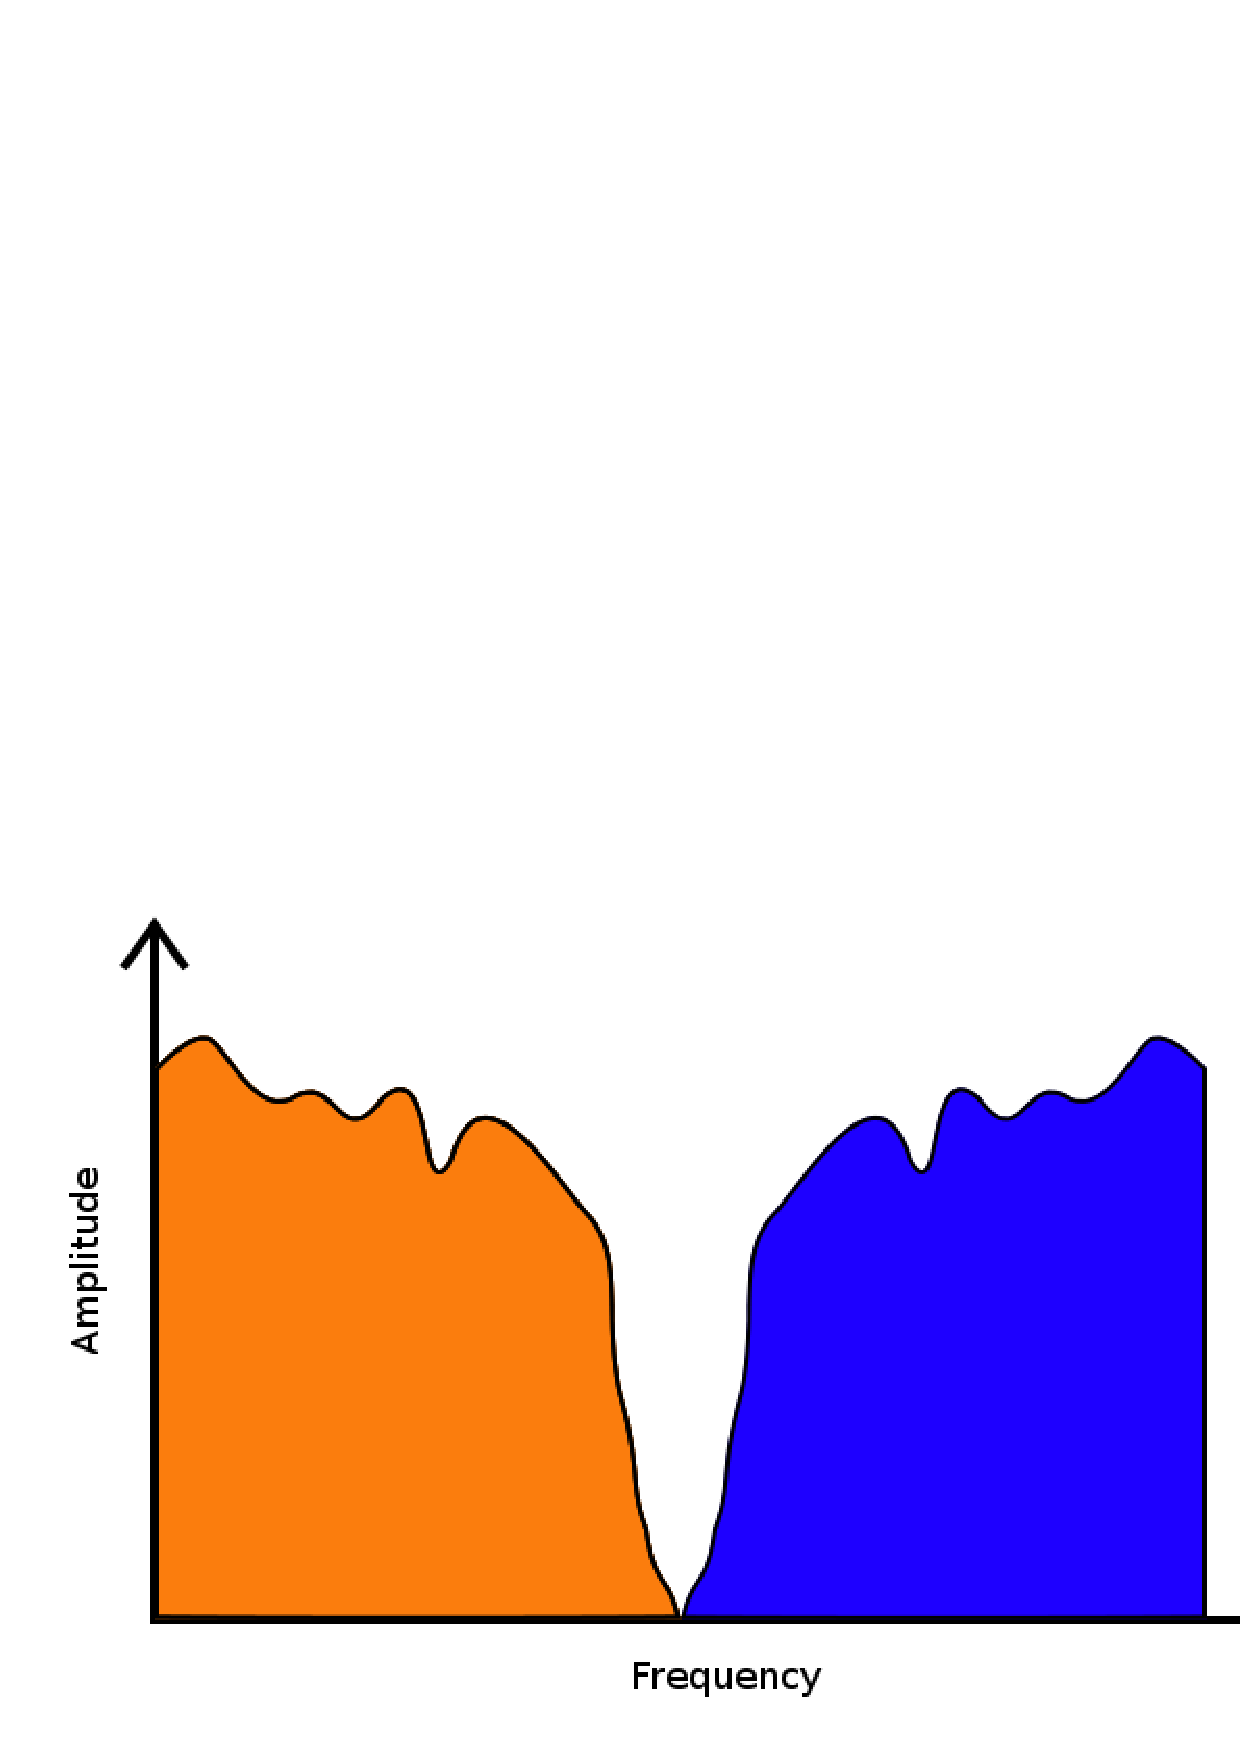
\includegraphics[width=0.4\textwidth]{Chapter3/Images/SpectralFolding.png}}
			\subfloat[Spectral Replication]{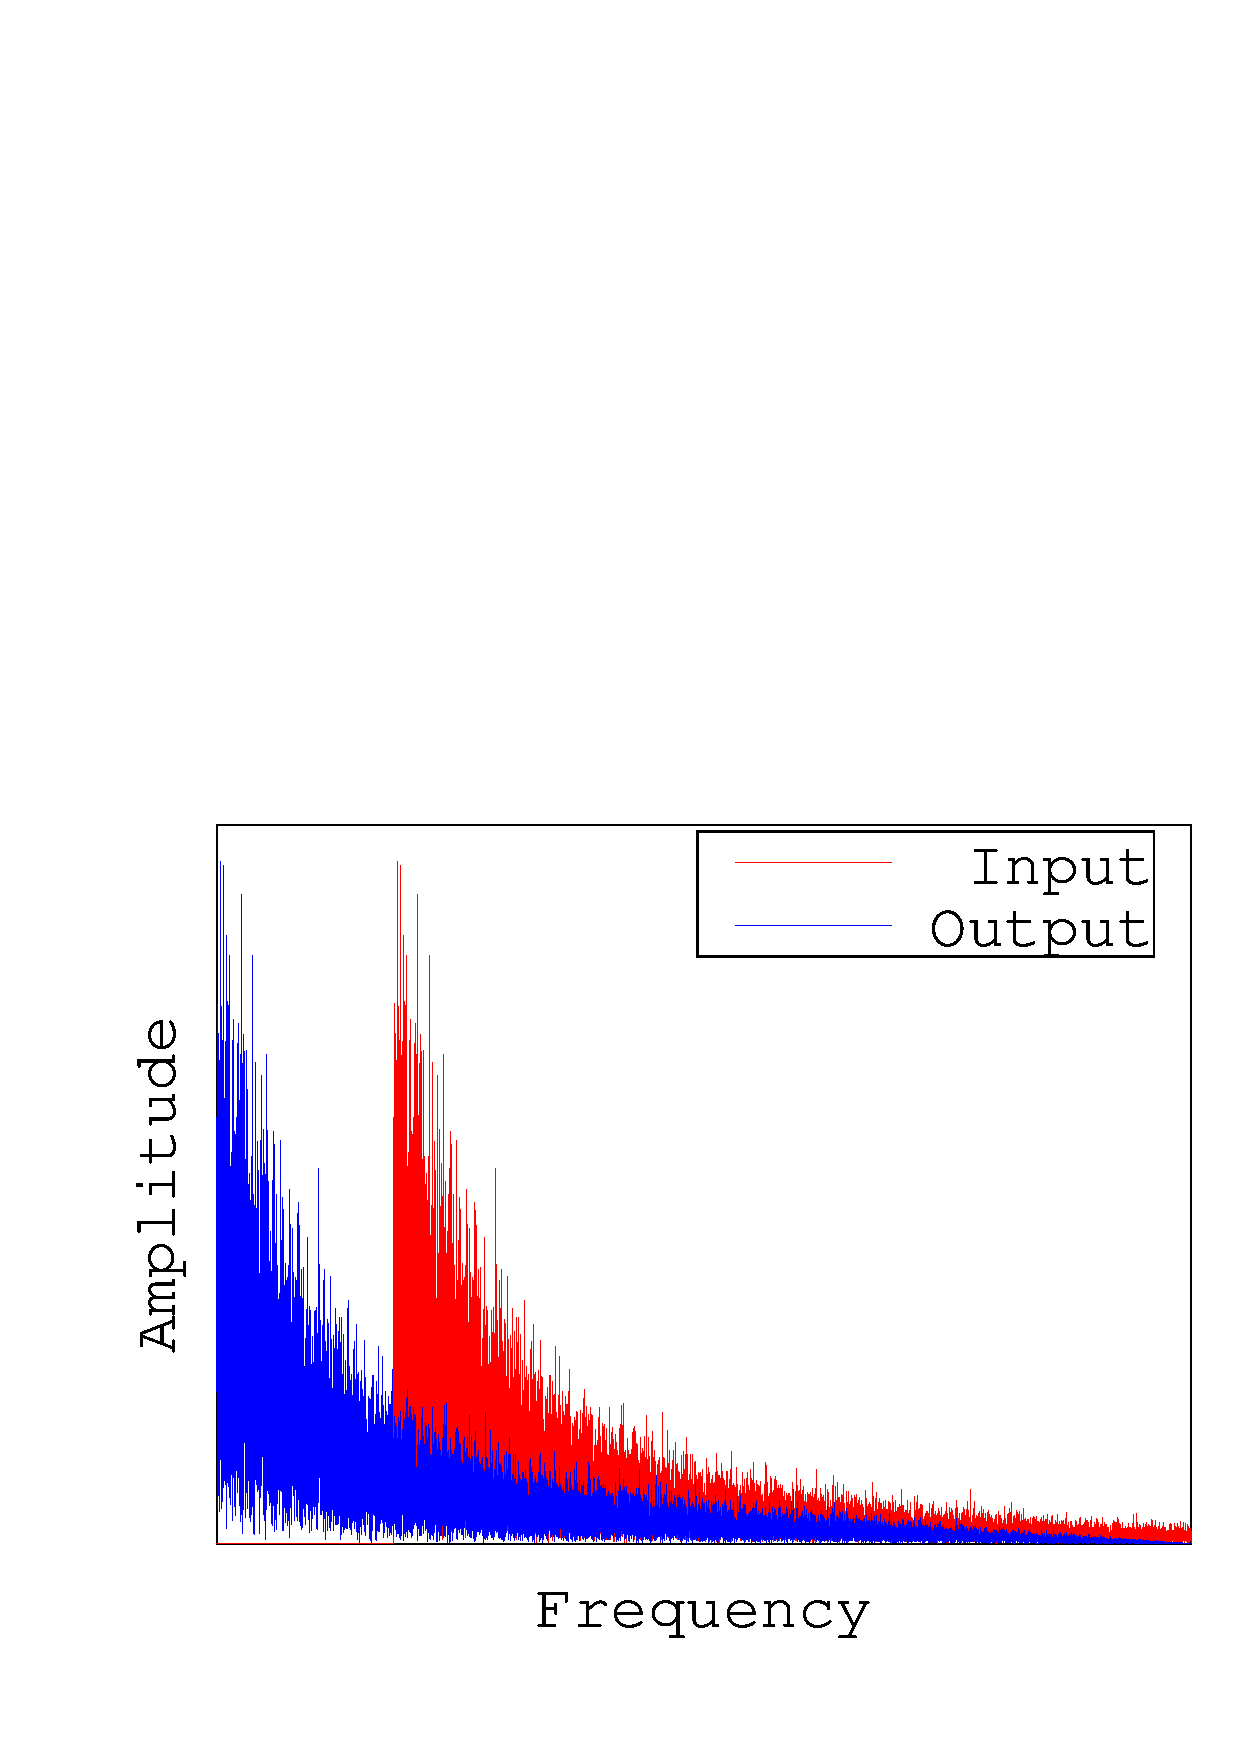
\includegraphics[width=0.4\textwidth]{Chapter3/Images/SpectralReplication.png}}
			\\
			\subfloat[Spectral Stretching]{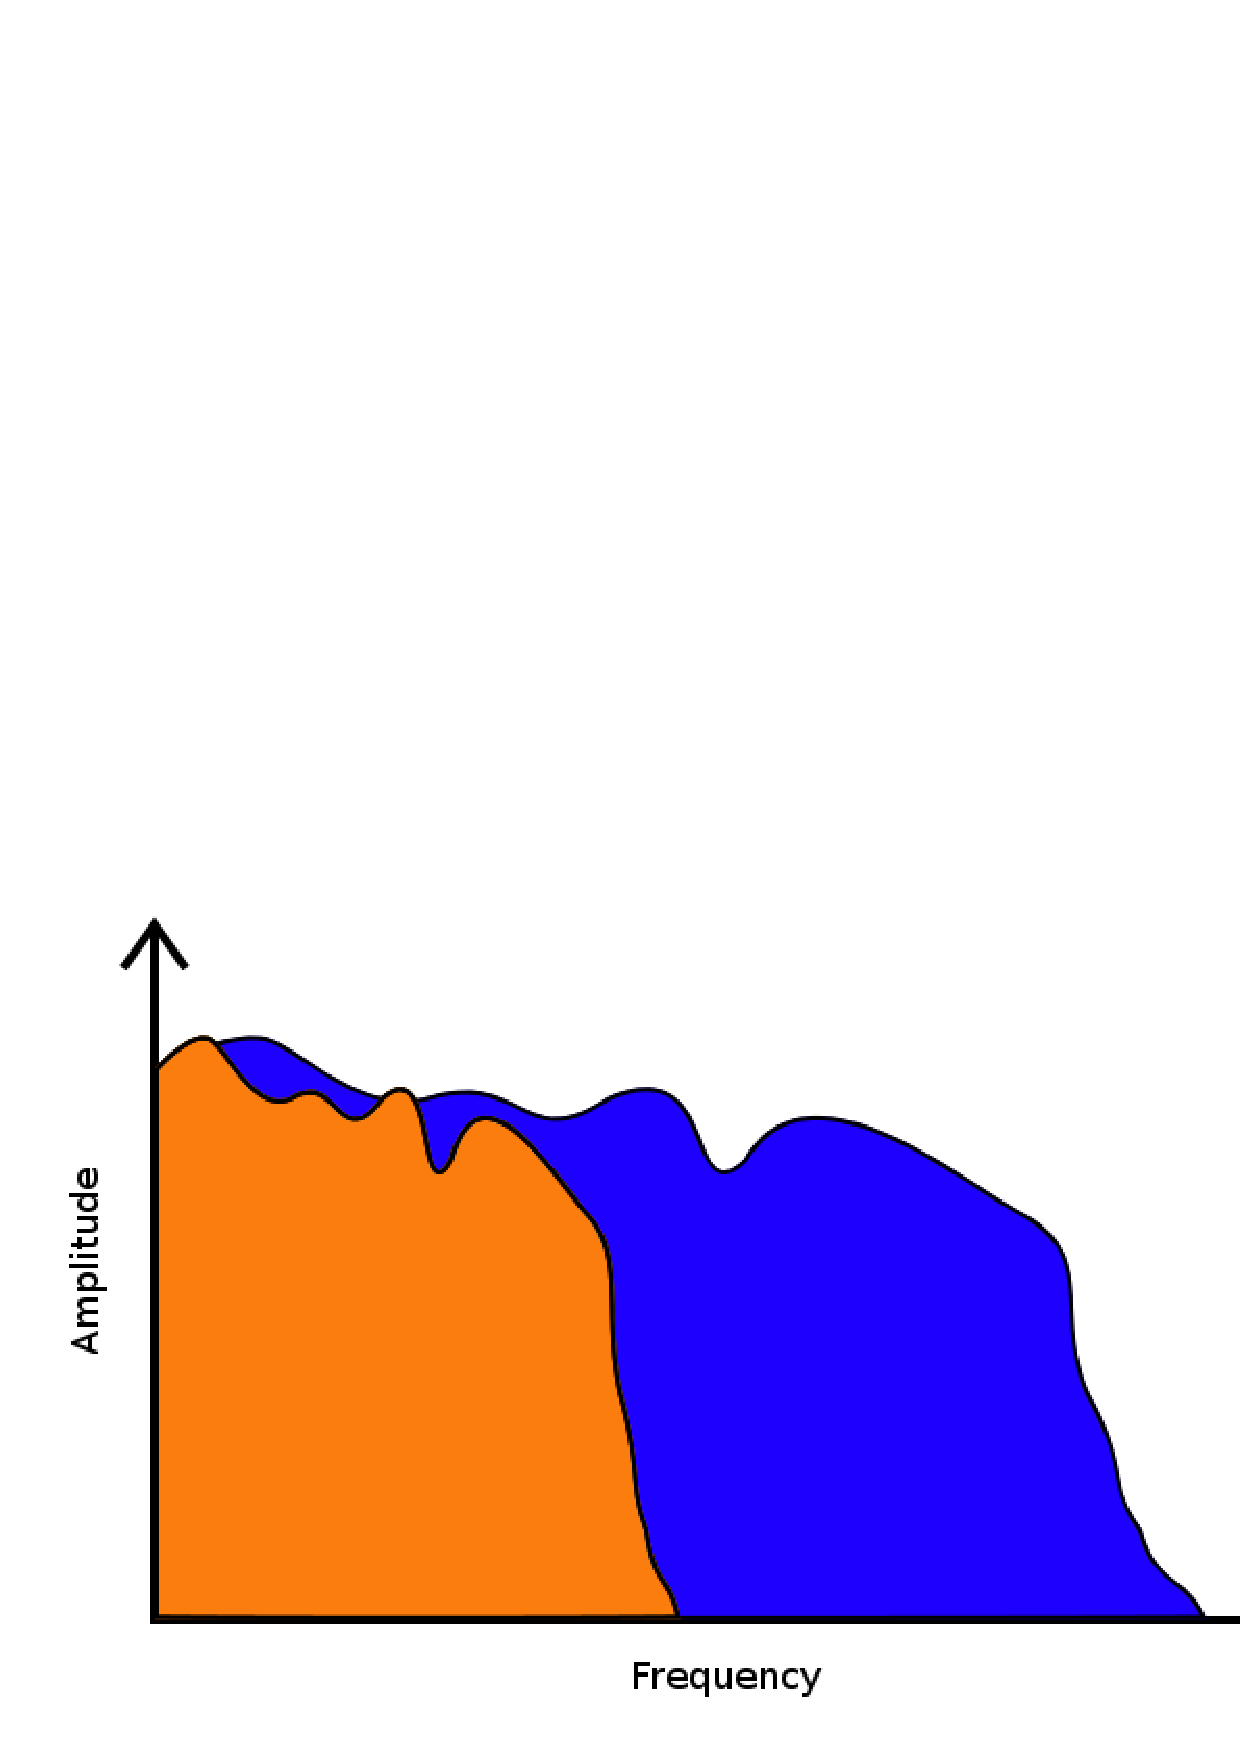
\includegraphics[width=0.4\textwidth]{Chapter3/Images/SpectralStretching.png}}
			\caption{Spectral characteristics of different band width extension methods. In each graph the blue section represents the original spectra and the red section the new spectral content.}
			\label{fig:SpectralFolding}
		\end{figure}

	\subsection{Individual Harmonic Generation}
	\label{sec:Excitation-Individuals}
		\note{SMC paper}

	\subsection{Psychoacoustic Enhancers}
	\label{sec:Excitation-Enhancers}
		\note
		{
			Probably the most well known perceptual control effects out there. The Aural Exciter has been covered by both \citet{chalupper2000aural} and \citet{shekar2013modeling}.
		}

	\subsection{Fundamental Frequency Tracking}
	\label{sec:Excitation-Fundamental}
		\note
		{
			Several generation methods can be improved through tracking the fundamental frequency of the input signal.

			We can talk all about fundamental / pitch tracking here \citep{cuadra2001efficient, gerhard2003pitch, prukkanon2009vt-amdf, larsen2004audio}.
		}
